\documentclass{article}
\usepackage[utf8]{inputenc}

\title{CS 376 : Assignment 6 \\
Modeling and Simulation of Petri Nets}
\author{Fred Eisele }
\date{29 October 2014}

\usepackage{natbib}
\usepackage{graphicx}

\begin{document}

\maketitle

\section{Introduction}
A tourist agency is setting up boat sightseeing tour
where the boats are autonomous vehicles.
You have been employed by the agency to design a control
system that drives the boat along the channels
as described in the following map.


\begin{figure}[h!]
\centering
\includegraphics[scale=0.5]{boat_tour.png}
\caption{Boat Tour}
\label{fig:boat-tour}
\end{figure}

\section{Single Boat Indeterminate Path}

Model the problem of a single boat with a Petri net
and describe in detail what each place and transition represents

\begin{figure}[h!]
\centering
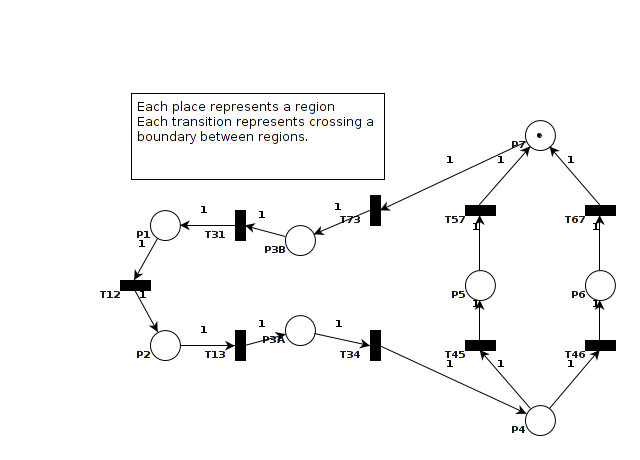
\includegraphics[scale=0.5]{hw6_petri_net_1.png}
\caption{Single Boat with Indeterminate Path}
\label{fig:pn1}
\end{figure}

\section{Single Boat Determinate Path}

Assume that the tourist agency wants that the
boat passes alternatively through sector 5 and 6.
Modify the Petri net in (a) so that this constraint is satisfied.

\begin{figure}[h!]
\centering
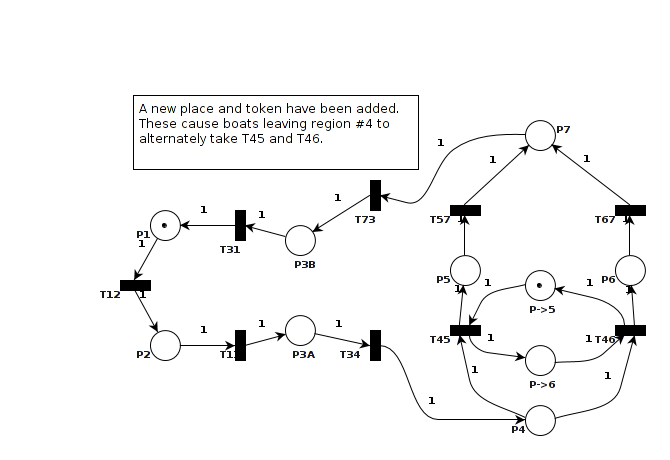
\includegraphics[scale=0.5]{hw6_petri_net_2.png}
\caption{Single Boat with Determinate Path}
\label{fig:pn2}
\end{figure}


\section{Two Boats Place Exclusion}

Assume there are two boats.
Specify a Petri net such that only one boat
can access sector 3 at a time.

\begin{figure}[h!]
\centering
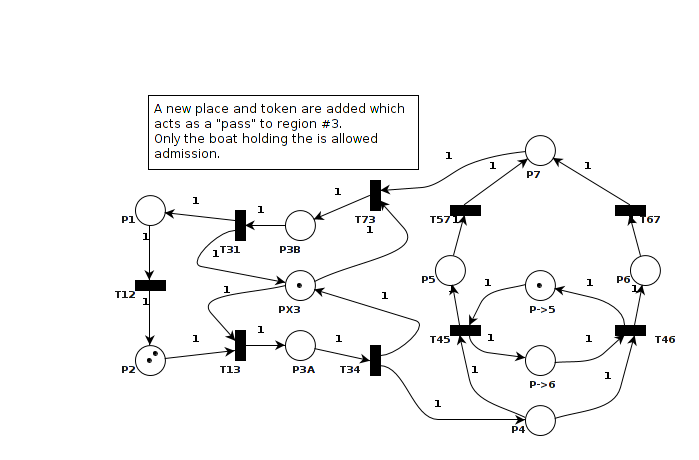
\includegraphics[scale=0.5]{hw6_petri_net_3.png}
\caption{Two Boat with Exclusion Zone and Determinate Path}
\label{fig:pn3}
\end{figure}

\end{document}
